\documentclass[11pt,ngerman,toc=listof,index=totoc]{scrreprt}
\usepackage{lmodern}
\usepackage{amssymb,amsmath}
\usepackage{ifxetex,ifluatex}
\usepackage{fixltx2e} % provides \textsubscript
\ifnum 0\ifxetex 1\fi\ifluatex 1\fi=0 % if pdftex
  \usepackage[T1]{fontenc}
  \usepackage[utf8]{inputenc}
\else % if luatex or xelatex
  \ifxetex
    \usepackage{mathspec}
  \else
    \usepackage{fontspec}
  \fi
  \defaultfontfeatures{Ligatures=TeX,Scale=MatchLowercase}
\fi
% use upquote if available, for straight quotes in verbatim environments
\IfFileExists{upquote.sty}{\usepackage{upquote}}{}
% use microtype if available
\IfFileExists{microtype.sty}{%
\usepackage{microtype}
\UseMicrotypeSet[protrusion]{basicmath} % disable protrusion for tt fonts
}{}
\usepackage{hyperref}
\hypersetup{unicode=true,
            pdfborder={0 0 0},
            breaklinks=true}
\urlstyle{same}  % don't use monospace font for urls
\ifnum 0\ifxetex 1\fi\ifluatex 1\fi=0 % if pdftex
  \usepackage[shorthands=off,main=ngerman]{babel}
\else
  \usepackage{polyglossia}
  \setmainlanguage[]{german}
\fi
\usepackage{graphicx,grffile}
\makeatletter
\def\maxwidth{\ifdim\Gin@nat@width>\linewidth\linewidth\else\Gin@nat@width\fi}
\def\maxheight{\ifdim\Gin@nat@height>\textheight\textheight\else\Gin@nat@height\fi}
\makeatother
% Scale images if necessary, so that they will not overflow the page
% margins by default, and it is still possible to overwrite the defaults
% using explicit options in \includegraphics[width, height, ...]{}
\setkeys{Gin}{width=\maxwidth,height=\maxheight,keepaspectratio}
\IfFileExists{parskip.sty}{%
\usepackage{parskip}
}{% else
\setlength{\parindent}{0pt}
\setlength{\parskip}{6pt plus 2pt minus 1pt}
}
\setlength{\emergencystretch}{3em}  % prevent overfull lines
\providecommand{\tightlist}{%
  \setlength{\itemsep}{0pt}\setlength{\parskip}{0pt}}
\setcounter{secnumdepth}{5}
% Redefines (sub)paragraphs to behave more like sections
\ifx\paragraph\undefined\else
\let\oldparagraph\paragraph
\renewcommand{\paragraph}[1]{\oldparagraph{#1}\mbox{}}
\fi
\ifx\subparagraph\undefined\else
\let\oldsubparagraph\subparagraph
\renewcommand{\subparagraph}[1]{\oldsubparagraph{#1}\mbox{}}
\fi
\usepackage[autostyle=true,german=quotes]{csquotes}
\usepackage{graphicx}
\usepackage{lmodern}
\usepackage{hyperref}
\usepackage[utf8]{inputenc}
\usepackage[T1]{fontenc}
%\usepackage{garamondx}
\usepackage[lf,p]{ebgaramond}
\usepackage{inconsolata}
\usepackage{titlesec}
\usepackage{fancyhdr}
\usepackage{color}
%\definecolor{titlepagecolor}{RGB}{122,153,1}
% \definecolor{titlepagecolor}{RGB}{253,246,227} %Solarized light background
% \definecolor{titlepagefontcolor}{RGB}{101,123,131} %Solarized light default text 
% \definecolor{titlepagecolor}{RGB}{84,153,224} %Solarized light background
\definecolor{titlepagecolor}{RGB}{40, 59, 84} 
\definecolor{titlepagefontcolor}{RGB}{225,225,225} %Solarized light default text 
\usepackage{ifthen}
\usepackage[usenames,dvipsnames]{xcolor}
\usepackage[
  paper=a4paper,
  left=25mm,
  right=25mm,
  top=21mm,
  bottom=25mm,
  includefoot,
  foot=\baselineskip,
  bindingoffset=0mm]{geometry}

\usepackage{setspace}
\onehalfspacing

\usepackage{amssymb}% http://ctan.org/pkg/amssymb
\usepackage{pifont}% http://ctan.org/pkg/pifont
\newcommand{\cmark}{\ding{51}}%
\newcommand{\xmark}{\ding{55}}%

\hypersetup{colorlinks,breaklinks,urlcolor=titlepagecolor,linkcolor=titlepagecolor}

\definecolor{gray75}{gray}{0.55}
\newcommand{\hsp}{\hspace{5pt}}

\titleformat{\chapter}      % Command 2
    [hang]                  % Shape
    {\Huge\bfseries}        % Format
    {\textcolor{titlepagecolor}{\thechapter\hsp|\hsp}}{0pt}
    {\Huge\bfseries}

\titleformat{\section}
    {\color{black}\normalfont\Large\bfseries}
    {\selectfont\color{titlepagecolor}\thesection\hsp|\hsp}{0em}{}

\titleformat{\subsection}
    {\color{black}\normalfont\large\bfseries}
    {\color{titlepagecolor}\thesubsection}{1em}{}

\titleformat{\subsubsection}
    {\color{black}\normalfont\bfseries}
    {\color{titlepagecolor}\thesubsubsection}{1em}{}

% Decrease Chapter Spacing.
\titlespacing{\chapter}{0pt}{0.0em}{2em}
\pagestyle{fancy}               

\newcommand{\prettypage}{%
    \scshape{~\thepage~~~}
}%

% Configure footer and header
\fancyfoot[C]{%
    % EasterEgg
    \ifthenelse{\value{page}=42}{%
        % Horizontal and vertical flip
        \reflectbox{\scalebox{1}[-1]{\prettypage}}
    }{%
        \ifthenelse{\value{page}=23}{%
            % Horizontal flip
            \reflectbox{\prettypage}
        }{%
            \prettypage
        }%
    }%
}%

% Remove the header from pages with chapters on them:
\fancypagestyle{plain}{%
    \fancyhead{}
    \renewcommand{\headrule}{}
}%

% \setlength{\headheight}{24pt} 

% Comment out for normal twoside:
% \newcommand{\ONESIDEFAKE}

\ifdefined\ONESIDEFAKE
    \fancyhead[L]{{\nouppercase{\slshape{\leftmark}}}}
    \fancyhead[R]{{\nouppercase{\scshape{\rightmark}}}}
\else
    \fancyhead[LO]{{\nouppercase{\slshape{\leftmark}}}}
    \fancyhead[RO]{{\nouppercase{\scshape{\rightmark}}}}
    \fancyhead[LE]{{\nouppercase{\scshape{\rightmark}}}}
    \fancyhead[RE]{{\nouppercase{\slshape{\leftmark}}}}
\fi

%\setlength{\topmargin}{-.5in}  %{-.5625in}
\setlength{\footskip}{25pt} % to put page number 3/4" from the bottom of the page (1/4" from bottom of body text)
%\setlength{\textheight}{9in}
%\setlength{\textwidth}{6in}

\date{\today}

\begin{document}

\begin{titlepage}
\pagecolor{titlepagecolor}
\begin{center}

\bf
% Upper part of the page. The '~' is needed because \\
% only works if a paragraph has started.
%\includegraphics[width=0.25\textwidth]{docs/pics/title.png}~\\[1cm]
\color{titlepagefontcolor}
\textsc{\huge Hochschule Augsburg}\\[1.5cm]
\textsc{\LARGE Usability engineering}\\[0.5cm]

\includegraphics[width=0.25\textwidth]{docs/pics/title.png}~\\[1cm]

% Title
\rule{\linewidth}{0.5mm}
{\Huge \bfseries Die Gnome Human Interface Guidelines\\[0.4cm] }
\rule{\linewidth}{0.5mm}

% Author and supervisor
\noindent
\begin{minipage}[t]{0.4\textwidth}
\begin{flushleft} \Large
\emph{Student:}\\
\textnormal{Christopher \textsc{Pahl}}
\end{flushleft}
\end{minipage}%
\begin{minipage}[t]{0.4\textwidth}
\begin{flushright} \Large
\emph{Dozenten:} \\
\textnormal{Prof.\ Dr. Christian \textsc{Märtin}} \\
\textnormal{M.Sc. Jürgen \textsc{Engel}} \\
\textnormal{M.Sc. Christian \textsc{Herdin}}
\end{flushright}
\end{minipage}

\vfill

% Bottom of the page
{\large \today}
\end{center}
\end{titlepage}
\nopagecolor

{
\setcounter{tocdepth}{2}
\tableofcontents
}
\listoffigures
\pagenumbering{arabic} \setcounter{page}{1}

\chapter{Vorwort}\label{vorwort}

Diese Studienarbeit gibt eine Einführung in den GNOME Desktop und den
dort gängigen Usability Richtlinien. Die Richtlinien sollen an
Beispielen aus dem GNOME Desktop beleuchtet werden und die dahinter
liegenden Ideen und Konzepte dargestellt werden. Der zweite, größere
Teil der Arbeit besteht darin eine vom Autor geschriebene Anwendung auf
diese Richtlinien hin zu überprüfen und die dahinterliegenden
Design--Entscheidungen aus Sicht eines Anwendungsentwickler kritisch zu
validieren.

Viele Bilder wurden direkt der Onlinepräsenz der \emph{GNOME Human
Interface Guidelines} entnommen. Für diese, wurde aus Gründen der
Übersichtlichkeit, auf einen separaten Quellenlink verzichtet und die
Quelle wurde nur mit \texttt{»Quelle:\ HIG«} gekennzeichnet. Bilder ohne
Quellenangabe stammen vom Autor selbst.

\chapter{Einleitung}\label{einleitung}

\section{Historisches zu GNOME}\label{historisches-zu-gnome}

GNOME ist eine auf unixoiden Betriebssystemen weit verbreitete
Desktopumgebung. Aufgrund der Natur von Open--Source--Software haben
sich über die letzten 15 Jahre mehrere größere Desktop--Oberflächen
herausgebildet, GNOME ist neben KDE eine der bekanntesten,
funktionsreichsten und auch ältesten (erstes offizielles Release im Jahr
1999). Aktuell ist der Desktop in der Version \texttt{3.18} verfügbar
und wird von vielen Linux--Distributionen wie Fedora\footnote{Bekannte
  Linux Distribution für technich versierte Anwender:
  \url{https://en.wikipedia.org/wiki/Fedora_Project}} als
Standard--Desktop ausgeliefert. Direkt nach der Installation sieht der
Desktop meist ähnlich wie in Abbildung \{\textbf{???}\} aus. Eine
Erklärung der Desktopfunktionsweise ist nicht Teil dieser Arbeit, zu
diesem Thema gibt es allerdings ausreichend Dokumentation\footnote{Siehe
  dazu beispielsweise: \url{https://www.youtube.com/watch?v=xu0VSKvfNEI}}.

Der gesamte Desktop samt allen Anwendungen ist dabei freie Software und
unter der \texttt{GPL}{[}1{]} lizenziert (beziehungsweise in Fall von
Bibliotheken als \texttt{LGPL}). Technisch basieren dabei weite Teile
des Desktops auf der Oberflächenbibliothek \texttt{GTK+} und der
Utility--Bibliothek \texttt{GLib}. Ursprünglich kommt \texttt{GTK+}
dabei aus dem \emph{GNU Image Manipulation Program} (kurz \emph{GIMP}),
was noch immer eine der bekanntesten Anwendungen des GNOME--Desktops
ist.

\includegraphics{docs/pics/gnome-screen.png} \{\#fig:gnome-screen\}

Finanziert wird das Projekt durch Spenden und der GNOME
Foundation\footnote{Mehr Informationen unter:
  \url{https://www.gnome.org/foundation/}}, einer nicht--kommerziellen
Vereinigung der Hauptentwickler und einiger Firmen wie
\emph{RedHat}\footnote{Mehr Informationen unter:
  \url{https://www.redhat.com/de}}, die die Entwicklung sponsern.

\section{Fokus von GNOME}\label{fokus-von-gnome}

Das Design eines gesamten Desktops ist verhältnismäßig schwierig.
Erschwert wird dies noch durch die Ziele auf die sich GNOME fokussiert
hat. Wikipedia{[}2{]} listet lose die folgenden Ziele:

Der Desktop muss\ldots{}

\begin{itemize}
\tightlist
\item
  \ldots{}konsistent gestaltet und visuell ansprechend sein.
\item
  \ldots{}behindertengerecht nutzbar sein.
\item
  \ldots{}auch auf mobilen Touchdevices mit begrenzten Ressourcen
  funktionieren.
\item
  \ldots{}komplett internationalisiert sein, das heißt in möglichst
  vielen Sprachen vorliegen.
\item
  \ldots{}effizient sowohl für Gelegenheitsnutzer\footnote{In diesem
    Fall überwiegend Maus und Touch--zentrierte Bedienung.}, als auch
  für erfahrene Nutzer\footnote{In diesem Fall überwiegend
    Tastatur--zentrierte Bedienung.} nutzbar sein.
\end{itemize}

Die oben stehenden Ziele werden durch die Arbeit vieler
Freiwilliger{[}3{]} relativ strikt für ca. 100 Kernanwendungen im GNOME
Desktop umgesetzt. Daneben gibt es noch eine Vielzahl weiterer
Anwendungen für speziellere Zwecke, welche diese Ziele mehr oder weniger
umsetzen. Dabei ist zu betonen, dass die meisten GNOME--Programme ---
anders als bei beispielsweise KDE --- auch ohne des Rest des
GNOME--Desktops lauffähig sind.

Das komplette Projekt als ganzes hat zudem noch weitere Ziele:

\begin{itemize}
\tightlist
\item
  Halbjährliche Releases mit Support von den Entwicklern.
\item
  In den Desktop integriertes und lokalisiertes Handbuch.
\item
  Entfernung von störenden und ablenkenden Design Entscheidungen.
\end{itemize}

Besonders der letzte Punkt ist oft Quelle von Kritik gegenüber dem
GNOME--Desktop, da darunter auch des Öfteren für versierte Nutzer
essentielle Konfigurationseinstellungen fallen. Das Ziel hier ist es
einerseits eine klare, minimale Oberfläche zu haben und andererseits
dadurch auch für Gelegenheitsnutzern die Bedienung einfacher zu
gestalten. Statt auf Kompromisse einzugehen, entfernen die GNOME--Macher
hier gemäß der Unix--Philosophie (\emph{Do (just) one thing and do it
well} {[}4{]}) alle Features, die nicht direkt dem Zweck der Anwendung
dienen. Die meisten Einstellungen sind allerdings für versierte Anwender
über die Kommandozeile erreichbar.

\chapter{GNOME Human Interface
Guidelines}\label{gnome-human-interface-guidelines}

Die GNOME Human Interface Guidelines versuchen die oben genannten
Probleme durch ein einheitliches Set von Richtlinien zu lösen, welches
jede Kernanwendung des GNOME--Desktops vollständig erfüllen muss.
Anwendungen rund um den Desktop (und auch externe Anwendungen) haben
keine so strikten Anforderungen, eine zumindest teilweise Einhaltung ist
aber wünschenswert.

Die Human Interface Guidelines{[}5{]} sind in fünf Hauptkapitel
gegliedert, die im Folgenden vorgestellt werden. Der Guide ist online
als HTML abrufbar.\footnote{siehe
  \url{https://developer.gnome.org/hig/stable/}} Oft wird der Guide als
\emph{der} \emph{\texttt{HIG}} abgekürzt, weswegen im Folgenden
hauptsächlich die Abkürzung zu lesen ist.

\section{\texorpdfstring{Prinzipien (\emph{Design
principles})}{Prinzipien (Design principles)}}\label{prinzipien-design-principles}

Die \emph{Prinzipien} des \texttt{HIG} definieren allgemeine
Grundgedanken. Diese sind nicht konkreter Natur, sondern geben nur eine
allgemeine Sammlung von Regeln und Tipps ab. Dies wird an einigen
Beispielen aus dem \texttt{HIG} deutlich:

\subsection{\texorpdfstring{\emph{Anticipate
errors}}{Anticipate errors}}\label{anticipate-errors}

Es wird empfohlen Fehler vom Nutzer zu erwarten und diese nach
Möglichkeit abzufangen. Als konkrete Maßnahme kommt für dieses
\emph{Prinzip} eine \emph{Undo} Funktionalität in Frage, um den Nutzer
die Möglichkeit zu geben auch destruktive (wie das Löschen von Items aus
einer Liste) Operationen rückgängig zu machen.

\subsection{\texorpdfstring{\emph{Prioritize
content}}{Prioritize content}}\label{prioritize-content}

Wichtigen Fensterinhalten sollte aller zur Verfügung stehender Platz
gegeben werden. Lediglich wichtige und in zu einem bestimmten Zeitpunkt
relevante Steuerelemente sollten noch parallel zu sehen sein. Dies führt
indirekt zu meist sehr übersichtlich gestalteten Oberflächen.

\subsection{\texorpdfstring{\emph{Avoid
interruptions}}{Avoid interruptions}}\label{avoid-interruptions}

Anwendungen die dem \texttt{HIG} folgen sollten möglichst Nutzer nicht
durch ablenkende Abfragen der Art \emph{»Sind sie sicher?«} ablenken.
Dies trifft insbesondere auf modale Popup--Dialoge zu, die eine
Benutzung des eigentlichen Programms unmöglich machen solange sie aktiv
sind.

Stattdessen wird empfohlen die Anwendung allgemein so zu gestalten, dass
der Nutzer von den Aktionen der Anwendung nicht überrascht ist, was eine
zusätzliche Abfrage unnötig macht.

\section{\texorpdfstring{Muster
(\emph{Patterns})}{Muster (Patterns)}}\label{muster-patterns}

Bei den sogenannten \emph{Mustern} wird es bereits konkreter. An dieser
Stelle gibt der Guide dem Entwickler eine Auswahl oft genutzter
Kombination von Designelementen an die Hand. Es wird dabei zwischen
vorgeschriebenen Mustern und situationsabhängig empfehlenswerten Mustern
entschieden.

Ein vorgeschriebenes Muster ist beispielsweise die \emph{Headerbar}
(siehe Abbildung \{\textbf{???}\}). Diese bietet Platz für viele
generische \emph{Elemente}, wie dem \emph{Suchmodus}, dem
\emph{Ansichtenswitcher} und dem \emph{Menübutton}.

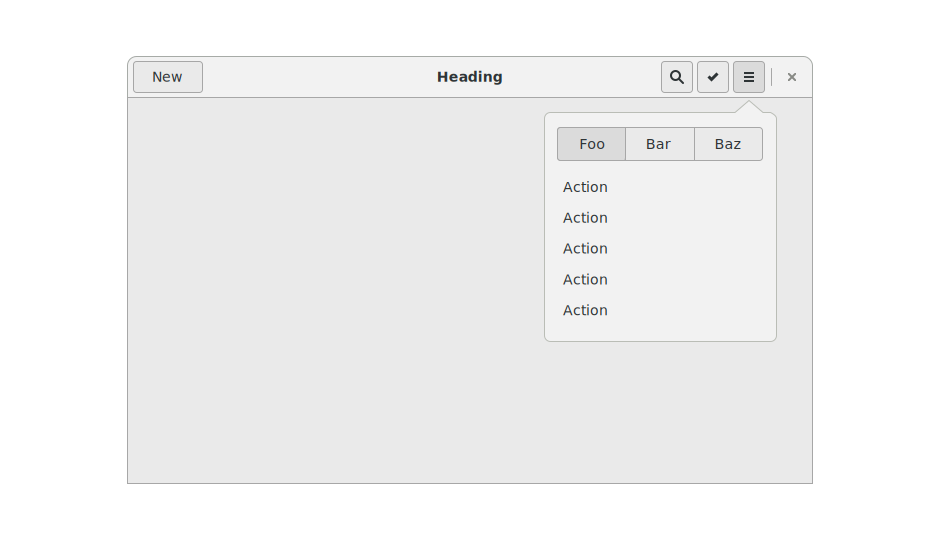
\includegraphics{docs/pics/headerbar.png} \{\#fig:headerbar\}

Bei vielen Anwendungen hingegen ist die \emph{Actionbar} eine gute, aber
optionale, Möglichkeit eine Liste von Aktionen für eine Auswahl
anzuzeigen. Dabei taucht nach der Auswahl von Text, Listenelementen oder
Ähnlichem am unteren Rand eine Bar mit unterschiedlichen Schaltflächen
auf, die jeweils einer Aktion zugeordnet sind. Einzelne dieser Aktionen
können dabei \textcolor{blue}{blau} (die empfohlene Aktion) oder
\textcolor{red}{rot} (gefährliche, destruktive Operation) hervorgehoben
sein. Dazu mehr im nächsten Kapitel.

\begin{figure}[htbp]
\centering
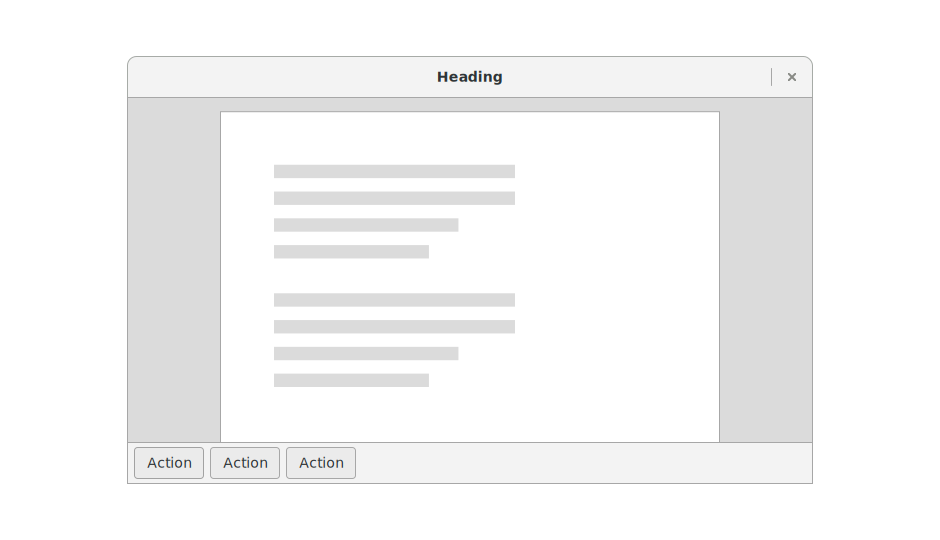
\includegraphics{docs/pics/actionbar.png}
\caption{Das \emph{Actionbar} Muster (Quelle: \texttt{HIG})}
\end{figure}

Im \texttt{HIG}\footnote{siehe
  \url{https://developer.gnome.org/hig/stable/patterns.html.de}} findet
sich eine weitaus größere Auswahl an weiteren Mustern. Zu jedem Muster
wird ein Beispielszenario und der empfohlene Einsatzzweck erläutert.

\section{\texorpdfstring{Elemente
(\emph{Elements})}{Elemente (Elements)}}\label{elemente-elements}

Für Anwendungsentwickler am interessantesten sind die konkreten
\emph{Elemente} die der \texttt{HIG} anbietet. Dabei handelt es sich um
individuelle, atomare Widgets oder Widgetgruppen, die ein gemeinsames
Ziel erfüllen. Meist handelt es sich dabei um alltägliche Bedienelemente
wie Menüs, Fortschrittsanzeigen und spezialisierte Schaltflächen. Von
den \emph{Patterns} unterscheiden sie sich dabei dadurch, dass sie
weniger allgemein sind und meist direkt einem Widget aus der
\texttt{GTK+}--Bibliothek entsprechen.

\includegraphics{docs/pics/elements.png} \{\#fig:elements\}

Ein häufig genutztes \emph{Element} ist beispielsweise der
\emph{Suggested Action Button}. Dabei handelt es sich um eine normale
Schaltfläche, die aber \textcolor{blue}{blau} hinterlegt ist. Er wird
per Konvention für alle Aktionen eingesetzt, von denen man erwartet,
dass der Nutzer sie am ehesten ausführen wird. Beispielsweise wäre eine
\texttt{Einstellungs}--Schaltfläche nicht \textcolor{blue}{blau}
hinterlegt, ein \texttt{Installieren} oder \texttt{Weiter}--Knopf
hingegen schon.

Im \texttt{HIG}\footnote{siehe
  \url{https://developer.gnome.org/hig/stable/ui-elements.html.de}}
findet sich eine noch weitaus größere Auswahl konkreter Elemente.

\section{\texorpdfstring{Anleitungen
(\emph{Guidelines})}{Anleitungen (Guidelines)}}\label{anleitungen-guidelines}

Die \emph{Guidelines} sind wieder etwas weniger konkret. Statt
ausschließlich das Aussehen der Anwendung zu beschreiben wird hier
beschrieben wie die Anwendung sich verhalten soll oder auf den Nutzer
wirken soll. Darunter fallen auch Tipps für gute Anwendungs--Namen und
Icons.

Beispielsweise finden sich dort auch Tipps zu folgenden Themen:

\subsection{\texorpdfstring{Beispiel:
\emph{Typografie}}{Beispiel: Typografie}}\label{beispiel-typografie}

Um visuell angenehme Anwendungen zu entwickeln sollte großen Wert auf
das Schriftbild gelegt werden. Beispielsweise sollten Schlüssel--Wert
Paare wie in Abbildung \{\textbf{???}\} der Lesbarkeit halber mittig
zentriert werden.

\includegraphics{docs/pics/align.png} \{\#fig:align\}

Auch Kleinigkeiten sollten dabei beachtet werden. So sollte eine
Bildschirmauflösung mit dem korrekten Unicode--Zeichen
(\texttt{U+d7,\ multiplication\ sign}) angezeigt werden, statt mit einem
einfachen \texttt{»x«}: 1024×768.

\subsection{\texorpdfstring{Beispiel: \emph{Touch
Gesten}}{Beispiel: Touch Gesten}}\label{beispiel-touch-gesten}

Der GNOME Desktop soll reibungslos auf mobilen Geräten benutzbar sein.
Daher sollten Anwendungsentwickler auf Touch--unfreundliche Eingaben wie
Doppelklicks verzichten und sicher stellen, dass typische Gesten wie das
»Zusammenziehen« mit den Fingern tatsächlich in ein Zoomen umgesetzt
wird.

\section{\texorpdfstring{Ressourcen
(\emph{Resources})}{Ressourcen (Resources)}}\label{ressourcen-resources}

Neben den tatsächlichen Richtlinien finden sich im GNOME Umfeld noch
einige allgemein nützliche Ressourcen. Darunter fällt beispielsweise das
\emph{Tango Icon Set} (siehe \{\textbf{???}\}), der freie
Cantarell--Font (siehe \{\textbf{???}\}) sowie das Tango--Colorscheme
(siehe \{\textbf{???}\}).

\includegraphics{docs/pics/cantarell.png} \{\#fig:tango-icons\}

\includegraphics{docs/pics/tango-icons.png} \{\#fig:cantarell\}

\chapter{Shredder --- Eine
Beispielanwendung}\label{shredder-eine-beispielanwendung}

Der \texttt{HIG} scheint für Außenstehende zunächst nur eine sehr
theoretische Richtlinie ohne praktische Relevanz für
Anwendungsentwickler zu sein. Um die tatsächliche Anwendbarkeit
begreifbarer zu machen wird in diesem Kapitel eine Beispielanwendung
durchleuchtet, die den \texttt{HIG} größtenteils implementiert.

\section{\texorpdfstring{Entstehung von
\emph{Shredder}}{Entstehung von Shredder}}\label{entstehung-von-shredder}

\begin{figure}[htbp]
\centering
\includegraphics{docs/pics/shredder_logo.png}
\caption{Das Logo von \emph{Shredder}.}
\end{figure}

\emph{Shredder} ist eine vom Autor im Jahr 2015 geschrieben Anwendung.
Sie bietet unter unixoiden Betriebssystemen die Möglichkeit doppelte
Dateien und Ordner zu finden und diese bei Bedarf auch zu löschen.
\emph{Shredder} ist in Python geschrieben und umfasst ca. 4000 Zeilen
Quellcode. Die eigentliche Arbeit des Duplikatesuchens erledigt dabei
das Kommandozeilenprogramm \texttt{rmlint} {[}5{]} im Hintergrund.

\texttt{rmlint} stammt ebenfalls vom Autor dieses Dokuments und umfasst
wegen des großen Feature--Umfangs ca. 9000 Zeilen C--Code, sowie eine
Python--Testsuite, die wiederum 3000 Zeilen umfasst. \texttt{rmlint}
selbst löscht keine Duplikate, schreibt aber nach erfolgreichen
Durchlauf ein \texttt{.sh}--Shellskript in eine Datei. Diese kann dann
vom Nutzer ausgeführt werden, um alle gefundenen Duplikate zu löschen.
Da \emph{Shredder} ein grafisches Frontend zu \texttt{rmlint} ist, setzt
es diesem Prozess ähnlich um, bietet dabei aber zusätzlich Interaktion
und Visualisierung.

Sowohl \emph{Shredder} als auch \texttt{rmlint} können unter
\url{http://rmlint.rtfd.org}{[}6{]} heruntergeladen werden. Unter
{[}7{]} findet sich zudem ein Video, welches die Benutzung von
\emph{Shredder} erklärt.

\section{\texorpdfstring{Programmstruktur von
\emph{Shredder}}{Programmstruktur von Shredder}}\label{programmstruktur-von-shredder}

\includegraphics{docs/pics/shredder_screen.png} \{\#fig:screen\}

\emph{Shredder} wurde größtenteils nach den Prinzipien des \texttt{HIG}
gestaltet. Die Bereiche in denen das Design vom Guide abweicht, werden
weiter unten beleuchtet. Das ursprüngliche Design ist stark von dem bei
Gnome mitgelieferten Programm \texttt{baobab}\footnote{\url{https://de.wikipedia.org/wiki/Baobab_(Software)}}
inspiriert, welches dazu dient die Größenaufteilung in einem
Verzeichnisbaum zu visualisieren.

Prinzipiell ist die Anwendung in unterschiedliche Ansichten aufgeteilt,
die den Nutzer, ähnlich wie ein \emph{Installations--Wizard}, durch den
Prozess des Duplikate--Entfernens führt. Dabei kann der Nutzer nach
Belieben zwischen den einzelnen Schritten wechseln und zwischen den
Ansichten hin- und her springen.

Zur Navigation dient dabei die \emph{Headerbar} (siehe Abbildung
\{\textbf{???}\}). Bei \emph{Shredder} finden sich in dieser links zwei
Schaltflächen, um die Ansichten der Reihe nach durchzuschalten. Die
Schaltflächen sind dabei in einer Box zusammengeschweißt. Der
\texttt{HIG} empfiehlt dieses \emph{Element} für Schaltflächen die eine
gegensätzliche Wirkung haben.

Rechts findet man eine Schaltfläche, um \emph{Shredder} in den Suchmodus
zu schalten (für mobile Anwender eine Alternative zu \texttt{STRG-F}).
Weiter rechts findet sich ein Menüknopf unter dem die Einstellungen und
der About--Dialog erreichbar ist.

Im Folgenden werden die einzelnen Ansichten nur grob besprochen. Eine
Erklärung sämtlicher Details würde den Umfang dieser Arbeit sprengen.

\subsection{\texorpdfstring{\texttt{Locations}
Ansicht}{Locations Ansicht}}\label{locations-ansicht}

\includegraphics{docs/pics/gui_locations.png} \{\#fig:locations\}

Nach dem Start wird zuerst die sogenannte \emph{Locations--Ansicht}
präsentiert (siehe \{\textbf{???}\}). Diese zeigt eine Liste von
möglichen Orten, die der Nutzer durchsuchen möchte. Standardmäßig
umfasst dies seinen \texttt{/home}--Ordner, das
\texttt{/var}--Verzeichnis\footnote{Hier werden unter Unix traditionell
  logs und caches abgespeichert.} und alle zuletzt unter GNOME genutzten
Verzeichnisse. Mit der \texttt{Add-Location}--Schaltfläche kann er auch
eigene Orte auswählen.

Der Nutzer kann dabei mit der Maus einzelne Ordner auswählen, die dann
\textcolor{blue}{blau} hinterlegt werden. Manchmal ist es nützlich
mehrere Ordner auszuwählen (beispielsweise \texttt{music} und
\texttt{music-copy}). Dabei möchte man dann oft nur die Duplikate in
einem der beiden Ordner löschen. Dies kann man erreichen, indem man den
\emph{Original}--Ordner mittels der Checkbox auf der rechten Seite als
solchen markiert. Im Beispiel würde der Nutzer beispielsweise
\texttt{music} als Original--Ordner kennzeichnen. Ist die selbe Datei in
\texttt{music} und \texttt{music-copy} vorhanden, so wird diese immer
nur aus \texttt{music-copy} gelöscht. Original--Ordner werden visuell
mit einem Karo--Hintergrund gekennzeichnet.

Wurde mindestens ein Ordner ausgewählt wird am unteren Rand eine
\emph{Actionbar} angezeigt mit welcher der Nutzer den Scanvorgang
starten kann. Da dies der wahrscheinlichste nächste Schritt des Nutzers
ist, wird die Schaltfläche \texttt{Scan\ folders} als \emph{Suggested
Action} in \textcolor{blue}{blau} hervorgehoben.

\subsection{\texorpdfstring{\texttt{Runner}
Ansicht}{Runner Ansicht}}\label{runner-ansicht}

\includegraphics{docs/pics/gui_runner.png} \{\#fig:runner\}

In der \texttt{Runner}--Ansicht werden in Echtzeit alle gefundenen
Duplikate angezeigt. Die Ansicht ist dabei zweigeteilt: Links findet
sich eine Baumansicht, welche die Pfade zu den Duplikaten abbildet.
Neben den einzelnen Pfaden wird noch die Größe der jeweiligen Datei oder
des Ordners angezeigt, sowie der Zeitpunkt der letzten Änderung und die
Anzahl der doppelten Dateien (bei Ordnern die Anzahl der Dupletten
darin). Vor dem eigentlichen Pfad wird zudem ein
\textcolor{green}{\cmark} oder ein \textcolor{red}{\xmark} angezeigt.
Dieses gibt Auskunft darüber, ob die Datei im nächsten Schritt gelöscht
wird. Durch ein Rechtsklickmenü kann der Nutzer diesen Zustand ändern.
\emph{Shredder} verhindert dabei gemäß dem oben erwähnten Prinzip
\emph{»Anticipate errors«} allerdings, dass sämtliche Duplikate samt den
Original mit einem \textcolor{red}{\xmark} markiert werden.

Auf der rechten Seite wird ein Kreisdiagramm gezeichnet, welches dem
Nutzer eine Vorstellung gibt, wo sich die meisten Duplikate finden. Das
Diagramm ist schichtenförmig aufgebaut. Auf der innersten Ebene findet
sich dabei als voller Kreis der gemeinsame Wurzelknoten aller
durchsuchten Ordner. Die darauf folgenden Ebenen sind dann jeweils die
Unterordner bzw. Dateien der Vorgängerebene. Dabei wird jedem
Unterordner je nach Menge und Größe von Duplikaten ein unterschiedlich
breites Kreissegment zugeordnet. Der Übersichtlichkeit halber werden
sehr kleine Segmente von der Darstellung ausgenommen, wodurch Lücken
entstehen.

Der Nutzer kann durch das Diagramm navigieren indem er die Maus über die
einzelne Segmente bewegt. Dabei wird der Name der Ordner auf derselben
Ebene als Tooltip eingeblendet (siehe auch {[}7{]}). Klickt er auf ein
Segment wird dies als neuer Wurzelknoten gesetzt. Dadurch können
Teilbäume der Hierarchie gesondert betrachtet werden.

Hat der Nutzer die dargebotene Sicht validiert, kann er mittels der
\texttt{Render\ Script}--Schaltfläche ein Shellskript generieren. Dabei
kann er durch die Dropdown--Liste rechts der Schaltfläche entweder alle
gefundenen Pfade in das Skript aufnehmen, oder alternativ nur alle
selektierten oder auch nur alle momentan sichtbaren. Sichtbar ist ein
Pfad wenn er durch eine Suchanfrage nicht gefiltert wurde
(\texttt{STRG-F}). Standardmäßig ist die Dropdown--Liste auf \emph{All}
voreingestellt.

\subsection{\texorpdfstring{\texttt{Editor}
Ansicht}{Editor Ansicht}}\label{editor-ansicht}

\includegraphics{docs/pics/gui_editor.png} \{\#fig:editor\}

In der \emph{Editor}--Ansicht wird das von \emph{Shredder} generierte
Shellskript mit Syntaxhighlighting angezeigt. Der Nutzer kann dieses
noch ein letztes Mal validieren. Erfahrene Nutzer können auch das Skript
editieren.

Diese Vorgehensweise mag erst einmal seltsam erscheinen, so soll aber
dem Nutzer die Angst vor dem ,,gefährlichen`` Vorgang des
Duplikate--Löschens genommen werden. Im Zweifelsfall kann er mit etwas
Recherche nachvollziehen was die Anwendung mit den gefundenen Dateien
tut. Uninteressierte Nutzer können hingegen gleich fortfahren, da es
sich dabei um keinen notwendigen Schritt handelt.

Das Skript kann durch die \texttt{»Run\ Script«}--Schaltfläche
ausgeführt werden. Dieser ist standardmäßig auf einen \emph{Trockenlauf}
(\texttt{»dry\ run«}) eingestellt. Klickt man in diesem Zustand auf die
\texttt{»Run\ Script«}--Schaltfläche, so wird das Skript bis auf die
tatsächlichen Lösch-Kommandos ausgeführt. Wenn der Nutzer
\emph{Shredder} ausreichend vertraut kann er zum tatsächlichen Löschen
übergehen, indem er den \texttt{»dry\ run«}--Teil der Schaltfläche
anklicken. Anschließend färbt sich die gesamte Schaltfläche rot und das
Warnungszeichen darüber verändert sich zu einem Totenkopf um den Nutzer
darauf aufmerksam zu machen, dass er jetzt destruktive Operationen
auslöst. Dies entspricht dem \texttt{HIG}--Prinzip \emph{»Use emotion
and humor (sparingly)«}.

\subsection{\texorpdfstring{\texttt{Settings}
Ansicht}{Settings Ansicht}}\label{settings-ansicht}

\includegraphics{docs/pics/gui_settings.png} \{\#fig:settings\}

Die Settings Ansicht findet sich \emph{links} von der zu Programmstart
gezeigten \emph{Locations}--Ansicht. Sie ist dabei entweder über die
Pfeile oben in der Headerbar erreichbar, oder über das Menü rechts in
der Headerbar.

In der eigentlichen Ansicht finden sich Gruppen von Schlüssel--Wert
Paaren. Jedem Schlüssel ist dabei eine deskriptive Beschreibung und ein
Widget auf der rechten Seite zugeordnet. Mit letzteren kann der Wert
verändert werden (siehe auch Abbildung \{\textbf{???}\}).

Wird einer der Werte geändert, taucht in der Headerbar ein
\texttt{Apply}- und eine \texttt{Reset}--Schaltfläche auf. Damit die
Änderungen tatsächlich übernommen werden, muss dieser betätigt werden.

\section{\texorpdfstring{Anwendungsbeispiele des
\texttt{HIG}}{Anwendungsbeispiele des HIG}}\label{anwendungsbeispiele-des-hig}

Oben wurden bereits einige Elemente genannt, die vom \texttt{HIG}
übernommen worden sind. Im Folgenden werden noch einige allgemeine
Grundgedanken genannt, die bei der Implementierung eine Rolle gespielt
haben.

\subsection{\texorpdfstring{Prinzip:
\emph{Durchsuchbarkeit}}{Prinzip: Durchsuchbarkeit}}\label{prinzip-durchsuchbarkeit}

Der \texttt{HIG} empfiehlt durch das Prinzip \emph{»Provide quick and
effective search«} die Anwendung zu jeder Zeit durchsuchbar zu machen,
um den Nutzer die Möglichkeit zu geben nur die Teile der Anwendung
anzuzeigen, die ihn interessieren.

Jede der oben genannte Ansichten kann vom Nutzer durchsucht werden,
indem er \texttt{STRG-F} drückt. Die Funktion der Suche unterscheidet
sich je nach Ansicht:

\begin{itemize}
\tightlist
\item
  \texttt{Settings}: Ein Konfigurationswert wird nur dann angezeigt,
  wenn in seinem Namen oder seiner Beschreibung ein Teil der Suchanfrage
  enthält.
\item
  \texttt{Locations}: Ein Ordner wird nur dann angezeigt wenn ein Teil
  seines Pfades die Suchanfrage enthält.
\item
  \texttt{Runner}: Hier filtert die Suche die angezeigten Duplikate.
  Neben einfachen Suchanfragen, die ähnlich wie bei \emph{Locations}
  nach Pfadkomponenten filtern, kann dem Suchbegriff ein Präfix wie
  \texttt{size:} mitgegeben werden, um (beispielsweise) nach der Größe
  zu filtern. Der Suchbegriff \texttt{»size:1M-4M«} würde dabei nur alle
  Duplikate mit einer Größe von ein bis vier Megabyte anzeigen. Weitere
  Präfixe sind \texttt{mtime:} für den letzten Änderungszeitpunkt und
  \texttt{count:}, was nach Anzahl der Zwillingsdateien filtert.
\item
  \texttt{Editor}: Das \texttt{.sh}--Dokument ist voll durchsuchbar. Es
  werden dabei pro Zeile alle Treffer angezeigt. Der Nutzer kann sich
  dabei mit dem Standard \texttt{GTK+}--Shortcut \texttt{STRG-G} durch
  die Treffer hangeln.
\end{itemize}

\subsection{\texorpdfstring{Prinzip: \emph{Keine
Unterbrechungen}}{Prinzip: Keine Unterbrechungen}}\label{prinzip-keine-unterbrechungen}

Auch bei Fehlern wird der Nutzer nicht durch Popup--Dialoge gestört.
Tritt beispielsweise ein Fehler beim Einlesen der Duplikate auf ---
beispielweise beim Einlesen eines Netzwerkmounts, welches plötzlich
verschwindet --- So wird dieser in einer \emph{In-app
Notification}\footnote{siehe
  \url{https://developer.gnome.org/hig/stable/in-app-notifications.html.de}}
unterhalb der \emph{Headerbar} angezeigt. Ist der Fehler nicht fataler
(aber erwähnenswerter) Natur kann der Nutzer diesen zur Kenntnis nehmen
und mit seiner Arbeit fortfahren.

\subsection{\texorpdfstring{Prinzip: \emph{Keine stockende
Oberfläche}}{Prinzip: Keine stockende Oberfläche}}\label{prinzip-keine-stockende-oberfluxe4che}

Die Oberfläche sollte zu jedem Zeitpunkt bedienbar bleiben. Insbesondere
sollten blockierende Operationen (wie das Suchen von Duplikaten)
keinesfalls die Anwendung stocken lassen. Der Anwender könnte dabei
denken, dass die Anwendung abgestürzt seie und deshalb beunruhigt die
Aktion abbricht.

Aus technischer Sicht muss daher Sorge getragen werden, dass
\texttt{GTK+} auch während blockierenden Operationen kurz Zeit bekommt
die Oberfläche neu zu zeichnen und Eingaben entgegennehmen.

\section{\texorpdfstring{Abweichungen vom
\texttt{HIG}}{Abweichungen vom HIG}}\label{abweichungen-vom-hig}

Teilweise weicht \emph{Shredder} mal mehr, mal weniger vom \texttt{HIG}
ab. In den meisten Fällen liegt das allerdings an noch nicht
implementierten Features.

\subsection{Detaillierte
Konfiguration}\label{detaillierte-konfiguration}

Ein Prinzip des \texttt{HIG} lautet \emph{»Use configuration options
sparingly«}. Dieses wird von \emph{Shredder} nicht direkt erfüllt.
Stattdessen bietet \emph{Shredder} dem Nutzer mittels der
\emph{Settings--Ansicht} eine große Auswahl von Stellschrauben. Nach
Meinung des Autors ist dies allerdings nötig, da das Finden von
Duplikaten keine leicht verallgemeinerbare Aufgabe ist. Der
,,Standardfall`` ist aber auch ohne zusätzliche Konfiguration
durchführbar.

Oben genanntes Prinzip ist nicht unumstritten. Oftmals wird die
mangelnde Konfigurierbarkeit von GNOME--Anwendungen kritisiert. Viele
Konfigurationswerte sind beispielsweise nur über die Kommandozeile
erreichbar. \emph{Shredder} geht hier einen Mittelweg: Es bietet dem
Nutzer mehr Stellschrauben, *,,versteckt``* diese aber in einer
gesonderten Ansicht. Diese Ansicht muss dabei als einziges beim
Duplikatefinden nicht durchlaufen werden.

Verbesserungswürdig hingegen wäre die Reihenfolge der
Konfigurationswerte. Zwar sind diese bereits nach Thema gruppiert,
allerdings könnte man diese auch noch nach Wichtigkeit sortieren.

\subsection{Handbuch und
Internationalisierung}\label{handbuch-und-internationalisierung}

Aufgrund von Zeitmangel des Autors enthält \emph{Shredder} leider noch
keine eingebautes Handbuch, auch wenn dieses vom \texttt{HIG} empfohlen
wird. Auch ist das Programm noch nicht in anderen Sprachen als Englisch
verfügbar, obwohl das dahinter stehende Programm \texttt{rmlint} bereits
in mehreren Sprachen vorliegt.

\subsection{Weitere kleinere
Abweichungen}\label{weitere-kleinere-abweichungen}

Es folgen der Vollständigkeit halber einige Details in denen
\emph{Shredder} noch vom \texttt{HIG} abweicht.

\subsubsection{Mobile Bedienbarkeit}\label{mobile-bedienbarkeit}

Zwar ist die Zahl der Nutzer auf mobilen Geräten vermutlich eher gering,
doch um für die Zukunft gewappnet zu sein, sollte \emph{Shredder} auch
mittels Touchgesten bedienbar sein. Dies funktioniert momentan für
einfache Anwendungsfälle, allerdings nicht für komplexere Anwendungen,
die beispielsweise das Rechtsklickmenü in der \emph{Runner}--Ansicht
benötigen. Der \texttt{HIG} erwähnt dabei die mobile Bedienbarkeit unter
den \emph{Guidelines} {[}8{]}.

\subsubsection{Anwendungsicon}\label{anwendungsicon}

Das Logo von \emph{Shredder} hält sich nicht strikt an die Vorgaben des
\texttt{HIG}, da das Logo bereits vor der Umsetzung von \emph{Shredder}
entstand. Insbesondere präferiert der \texttt{HIG} eckige Icons, die die
Tango Farbpalette benutzen (siehe Abbildung \{\textbf{???}\})

\includegraphics{docs/pics/tango.png} \{\#fig:tango\}

\subsubsection{Unintuitive Suchsyntax}\label{unintuitive-suchsyntax}

Es ist ohne Lesen des Manuals nicht ersichtlich, dass der Nutzer in der
\emph{Runner}--Ansicht Suchanfragen wie \texttt{size:4M} abgeben kann.
Eine mögliche Lösung wäre eine Dropdown--Liste wie in Abbildung
\{\textbf{???}\}. Diese würde alle möglichen Präfixe wie \texttt{size},
\texttt{mtime} und \texttt{count} anbieten. Beim Klick auf einen
Listenpunkt würde dann in das Suchfeld ein hervorgehobenes Textsnippet
wie \texttt{size:low-high} eingefügt werden. Dieses kann der Nutzer dann
editieren. Zudem werden momentan Syntaxfehler in der Suchsyntax nicht an
den Nutzer weitergegeben. Eine mögliche Lösung wäre den falschen Bereich
\textcolor{red}{rot} hervorzuheben.

\includegraphics{docs/pics/dropdown.png} \{\#fig:dropdown\}

\chapter{Fazit}\label{fazit}

Der Gnome \texttt{HIG} ist nur ein Ratgeber unter vielen. Viele andere
Anleitungen beziehen sich dabei meist auf Webanwendungen und nicht auf
Desktopanwendungen. Für viele Entwickler die keinen Design--Hintergrund
haben bietet der \texttt{HIG} daher eine detaillierte Hilfe, um schnell
und einfach gute Ergebnisse zu erzielen.

Im Gegensatz zu anderen Guides hat sich der \texttt{HIG} in der Praxis
bewährt und weit über 100 Programme befolgen ihn mit unterschiedlicher
Detailtreue.

Auch wenn man keine GNOME Anwendung entwickelt, kann der \texttt{HIG}
nützlich sein, da er Patterns für oft genutzte Designfragen bereithält.
Auch die Icons- und Fonts- Kategorie der Guidelines sind für externe
Projekte nützlich. Der \texttt{HIG} ist auch dann nützlich wenn man
nicht die technische Grundbasis und Bibliotheken von GNOME nutzt, da er
allgemein genug geschrieben ist. Wenn man ein anderes Toolkit als
\texttt{GTK+} nutzt ist das Nachbauen der einzelnen Widgets eventuell
schwieriger, aber die dahinter liegenden Paradigmen sind übertragbar.

\emph{Shredder} entspricht den meisten Prinzipien des \texttt{HIG}, auch
wenn nicht alle erwähnt worden sind. In der Zukunft sollten die
abweichenden Punkten nach Möglichkeit noch angeglichen werden.

\newpage

\chapter*{Literaturverzeichnis}\label{literaturverzeichnis}
\addcontentsline{toc}{chapter}{Literaturverzeichnis}

\hypertarget{refs}{}
\hypertarget{ref-gpl}{}
{[}1{]} R. Stallmann and others, ``GPL Licenses,'' 2015. {[}Online{]}.
Available: \url{https://www.gnu.org/licenses/gpl.html}.

\hypertarget{ref-wikiux5fgnome}{}
{[}2{]} W. authors, ``GNOME Desktop Environment,'' 2015. {[}Online{]}.
Available: \url{https://de.wikipedia.org/wiki/Gnome}.

\hypertarget{ref-german2003gnome}{}
{[}3{]} D. M. German, ``The GNOME project: a case study of open source,
global software development,'' \emph{Software Process: Improvement and
Practice}, vol. 8, no. 4, pp. 201--215, 2003.

\hypertarget{ref-raymond2003basics}{}
{[}4{]} E. Raymond, ``Basics of the Unix Philosophy,'' \emph{Als
Online-Dokument: http://www.faqs.org/docs/artu/ch01s06.html\#id2877537},
2003.

\hypertarget{ref-hig}{}
{[}5{]} G. Foundation, ``The Gnome Human Interface Guidelines,'' 2015.
{[}Online{]}. Available: \url{https://developer.gnome.org/hig/stable/}.

\hypertarget{ref-rmlint}{}
{[}6{]} C. Pahl, ``Rmlint Website,'' 2015. {[}Online{]}. Available:
\url{https://rmlint.readthedocs.org/en/latest/}.

\hypertarget{ref-shredderux5fvideo}{}
{[}7{]} C. Pahl, ``Shredder usage video,'' 2015. {[}Online{]}.
Available: \url{https://vimeo.com/139999878}.

\hypertarget{ref-mobile}{}
{[}8{]} G. Foundation, ``Pointer and Touch Input,'' 2015. {[}Online{]}.
Available:
\url{https://developer.gnome.org/hig/stable/pointer-and-touch-input.html.de}.

\end{document}
